\documentclass[letterpaper, 10 pt, conference]{IEEEconf}
\usepackage[utf8]{inputenc}
\usepackage[T1]{fontenc}
\usepackage[style=ieee]{biblatex}
\usepackage{tikz}
\usetikzlibrary{positioning,fit,arrows.meta,backgrounds}
\usepackage{amsmath, amssymb, xcolor, tikz, pgfplots, pgfplotstable}

\newcommand{\todo}[1]{{\color{red}#1}}
\usepackage{listings, xcolor}

\colorlet{punct}{red!60!black}
\definecolor{background}{HTML}{EEEEEE}
\definecolor{delim}{RGB}{20,105,176}
\colorlet{numb}{magenta!60!black}

\lstdefinelanguage{json}{
    basicstyle=\normalfont\ttfamily,
    numbers=left,
    numberstyle=\scriptsize,
    stepnumber=1,
    numbersep=8pt,
    showstringspaces=false,
    breaklines=true,
    frame=lines,
    backgroundcolor=\color{background},
    literate=
     *{0}{{{\color{numb}0}}}{1}
      {1}{{{\color{numb}1}}}{1}
      {2}{{{\color{numb}2}}}{1}
      {3}{{{\color{numb}3}}}{1}
      {4}{{{\color{numb}4}}}{1}
      {5}{{{\color{numb}5}}}{1}
      {6}{{{\color{numb}6}}}{1}
      {7}{{{\color{numb}7}}}{1}
      {8}{{{\color{numb}8}}}{1}
      {9}{{{\color{numb}9}}}{1}
      {:}{{{\color{punct}{:}}}}{1}
      {,}{{{\color{punct}{,}}}}{1}
      {\{}{{{\color{delim}{\{}}}}{1}
      {\}}{{{\color{delim}{\}}}}}{1}
      {[}{{{\color{delim}{[}}}}{1}
      {]}{{{\color{delim}{]}}}}{1},
}


\title{\LARGE \bf
A Pipeline for Assembling Collision and Near-Collision Dashcam Footage Datasets
}

\author{
         Ben Upenieks, Chaitanya Varier,\\
         Curtis Duy Kha Phan, Jack David Roberts Williamson,\\
         Nicholas Geofroy, Tony Meng, Vincent-Olivier Roch\\
         University of Waterloo\\
         \\
         \tt\small ben.upenieks@uwaterloo.ca, cvarier@uwaterloo.ca,
         \\ \tt\small cdkphan@uwaterloo.ca, jdrwilli@uwaterloo.ca,
         \\ \tt\small nicholas.geofroy@uwaterloo.ca, c24meng@uwaterloo.ca, vroch@uwaterloo.ca
}

\bibliography{sources}
\begin{document}

\maketitle
\thispagestyle{empty}
\pagestyle{empty}


%%%%%%%%%%%%%%%%%%%%%%%%%%%%%%%%%%%%%%%%%%%%%%%%%%%%%%%%%%%%%%%%%%%%%%%%%%%%%%%%
\begin{abstract}

The international movement towards developing autonomous vehicle technologies has raised concerns in many spheres of society: from legal perspectives \cite{Pattinson2020} to ethical dilemmas; from control theory to safety engineering; from cybersecurity to realtime computing. Over the
last decade, some emphasis has been made on the need for these vehicles to reduce road collisions and reckless driving. However, research into collision avoidance has been slowed down by the lack of egocentric footage datasets. Currently, this type of data is created through computer generated scenarios \cite{Kim_Lee_Hwang_Suh_2019} due to the dangerous and costly nature of road collisions. We provide a pipeline to assemble datasets of real events that have been published online to complement already existing methods. Futher, we present an aggregated dataset that we have produced using our pipeline which includes egocentric vehicle footage from all over the world subject to varying visibilities, varying weather conditions, and varying settings.

\end{abstract}

%%%%%%%%%%%%%%%%%%%%%%%%%%%%%%%%%%%%%%%%%%%%%%%%%%%%%%%%%%%%%%%%%%%%%%%%%%%%%%%%
\section{INTRODUCTION}

In the advent of connected vehicles and autonomous transportation, it has become commonplace to equip vehicles with the necessary equipment to facilitate high-end automated collision avoidance systems \cite{Perumal2020LidarBI}.
Using these vehicles to simulate collision situations has a two-fold cost: both the car and expensive data-gathering equipment are put at risk.
However, we can collect collision data naturally in real driving scenarios through the use of dashcams - cheap video cameras that can be mounted to a car's dashboard.
Typically used for insurance purposes, dashcams have the added benefit of recording a wide variety of collisions that wouldn't be feasible to simulate. 
This has led to the creation of many online communities to share videos of these rare situations on websites such as Reddit, YouTube, and Imgur.
We propose that this egocentric dashcam video stream can be leveraged by computer vision systems to act as an affordable and commonplace sensor for automated collision prediction. 

In this paper we present a software pipeline to facilitate the collection, processing and annotation of egocentric dashcam videos from various online video repositories to produce datasets that can be used to train deep dashcam collision prediction models.
We aim to generate datasets that are not constrained to any regions or countries but rather provide location-agnostic data that is representative of general, global road and vehicle conditions.
These datasets will also be collision-oriented as the majority of these videos contain collisions for people's viewing.
Current autonomous vehicle data collection techniques typically require astronomically expensive hardware and equipment and, consequently, are rarely involved in collisions and intentionally not put in high risk environments that may lead to a collision.
This is the data we hope to capture by taking advantage of existing videos of non-artificial collisions.

The pipeline uses web-scraping techniques to fetch the video data from these websites, along with a set of video metadata, describing the video's contents.
We use this data, in combination with the manually annotated data in order to create the collision dataset.
This combination allows us to take advantage of the wide variety of videos available on the internet, while still having reliable data that has been curated manually.
As part of this data, we identify participants and bystanders, both known as agents. Participants are objects that are involved in a collision identified in the metadata, while bystanders are objects that are not.

%%%%%%%%%%%%%%%%%%%%%%%%%%%%%%%%%%%%%%%%%%%%%%%%%%%%%%%%%%%%%%%%%%%%%%%%%%%%%%%%
\section{RELATED WORK}

Chan et al. \cite{chan2016anticipating} approach the same problem of collision prediction via egocentric dashcam videos. They propose a novel Dynamic-Spatial-Attention Recurrent Neural Network (DSARNN) that distributes attention to localized and detected vehicles within the video and models temporal dependencies to predict the earliest frame of a potential impending collision. Released with their paper is a dataset of 678 dashcam videos capturing areas in Taiwan. Each video is annotated with vehicle tracking bounding boxes, the vehicles that were involved in the collision and the frame of the collision. We hope to allow researchers to expand on this dataset with location-agnostic data and similar annotations.



%%%%%%%%%%%%%%%%%%%%%%%%%%%%%%%%%%%%%%%%%%%%%%%%%%%%%%%%%%%%%%%%%%%%%%%%%%%%%%%%
\section{METHODOLOGY}

The software pipeline is built of multiple executors that each process or handle the data corresponding to a single video before piping the resulting data to the next executor.


\begin{figure}[htpb]
		\centering
    \tikzset{
        module/.style={%
            draw, rounded corners,
            minimum width=#1,
            minimum height=7mm,
            font=\sffamily
            },
        module/.default=2cm,
        >=LaTeX
    }
    \begin{tikzpicture}[
      % This will show the frame around the figure
      show background rectangle]

      % Place first 6 items
      \node[module] (crawler) {Web-Scrapers};
      \node[module, below=of crawler] (downloader) {Downloaders};
      \node[module, below=of downloader] (splitter) {Video-Splitter};
      \node[module, below=of splitter] (labeller) {Video-Labelling Tool};
      \node[module, below=of labeller] (uploader) {Data-Uploader};
      \draw[->] (crawler)--(downloader);
      \draw[->] (downloader)--(splitter);
      \draw[->] (splitter)--(labeller);
      \draw[->] (labeller)--(uploader);

    \end{tikzpicture}
		\caption{Architecture of the default pipeline}
		\label{fig:obj-by-class}
\end{figure}


\subsection{Video Collection}

The entry into our pipeline is a set of web scraper executors that each target and scrape a specific website or video repository based on a user-defined set of key-terms, and a \textit{database source executor} that pulls unlabelled videos from the user's database. Videos that are pulled by the scrapers are immediately added to the database with relevant metadata and marked as unlabelled. Subsequently, they are loaded into memory and sequentially fed into the pipeline. If the pipeline terminates before labelling a video, it remains flagged as unlabelled in the database and the video will be pulled in a subsequent run by the \textit{database source executor}. Crawler state is maintained via database lookup of specified key-value pairs to ensure duplicate data is not pulled. No video preprocessing such as resizing, trimming or cropping is automatically performed.

Users may define their own search terms to be used when querying the video repository. This value can be set in a YAML pipeline configuration file. By default, our scrapers query using the keywords: \texttt{Car crash dashcam}. Currently we support crawling Reddit and YouTube to locate videos that are of interest, and downloading videos hosted on YouTube and Imgur. Users that want to pull from a video repository that is not currently implemented should create a custom executor and implement the \texttt{iCrawler} interface. This new executor should be added as an entry point in a new YAML configuration and should generate and return a \texttt{MetaDataItem} with video source information to be used by a subsequent and corresponding downloader. \texttt{MetaDataItem} objects are fed into the \texttt{UniversalDownloader} which aggregates \texttt{iDownloader} implementations and distributes \texttt{MetaDataItem} objects to their corresponding downloader via regular expressions matching of source URL's. New downloaders should be registered with the \texttt{UniversalDownloader} via a YAML pipeline configuration along with a regular expression string for URL matching.

%HAS BEEN REMOVED BECAUSE NOT FUNCTIONAL
%\subsection{Video Preprocessing}
%\subsection{Automatic Annotation}
%\subsection{Object Detection \& Tracking}
%\todo{Automated object detection not used right now?}
\subsection{Anonymization}
An important facet of automobile data aggregation is in eliminating biases and protecting the identities of depicted individuals. Consequently, our pipeline contains a post-processing stage in which we apply blurring masks to anonymize any personally identifiable information. Specifically, we provide the executor \texttt{FaceBlurrer}, which blurs faces. This executor first uses a MobileNet Single Shot MultiBox Detector \cite{yixuan_h_y_hu_2021_4642275} trained on the WIDERFACE dataset \cite{yang2016wider} to obtain the bounding boxes of all visibly identifiable individuals' faces at each frame of a given video and then applies a blurring mask over each bounding box.

This software module is encapsulated as a library and can be reused by importing our \texttt{anonymization} package. The accuracy, amount and type of blurring applied can be tweaked using the API exposed by the \texttt{anonymization} package.

\subsection{Annotation}

In addition to collection and preprocessing, a core component of our pipeline is a GUI tool that facilitates the manual annotation of the dashcam videos, and quick manual filtering of non-dashcam and irrelevant videos. Following Chan et al.\cite{chan2016anticipating}, if a collision occurs we provide tools to annotate the frame the collision occurs, and bounding boxes to localize, identify and track agents in the video segment. Object tracking bounding boxes can be linearly interpolated from manual start and end points to improve ease of labelling. We also save the video resolution at which the video was annotated to ensure bounding box annotations can always be scaled to fit any variable download resolutions. For long-form videos that may contain multiple collision events or irrelevant video segments, such as compilation videos or videos with substantial editing and transitions, we provide a video clipping feature to demarcate the collision events from which we extract and generate distinct data points. 
Each video segment will eventually become a metadata item. 

\subsection{Metadata}
After all of the previous steps have been completed, the pipeline is able to produce a complete metadata object.
There are many fields in the metadata object (as can be seen in Figure \ref{metadata_example}):

\begin{itemize}
  %\item "collision\_type" contains the type of collision in the video (e.g. car vs. car)
  \item "\texttt{description}" contains a description of the video as scraped from the video hosting website
  \item "\texttt{state}" is a string that describes the current state of the video. One of \textit{processed}, \textit{in-progress}, \textit{NULL}
  \item "\texttt{download\_src}" contains the site that the video was sourced from (e.g. YouTube)
  \item "\texttt{tags}" is an object that contains custom user-defined tags on videos and additional data that is site specific
  \item "\texttt{title}" is a string that represents the type of the video
  \item "\texttt{url}" is the url that the video was fetched from
  \item "\texttt{is\_split\_url}" is a boolean that is true if all of the frames of the video are covered in this metadata item and false if no
  \item "\texttt{enum\_tags}" is a list of tags identifying the content of the video. New tags can be added while labelling and can identify anything important in the video.
  \item "\texttt{start\_i}" is the start frame of the video that the bounding boxes are created for (if is\_split\_url is true)
  \item "\texttt{end\_i}" is the end frame of the video the bounding boxes are created for (if is\_split\_url is true)
  \item "\texttt{bb\_fields}" contains all bounding-box specific data
  \begin{itemize}
    \item "\texttt{collision\_locations}" is a list of frame numbers indicating the collision start frames
    \item "\texttt{resolution}" is a list with 2 elements (Width,Height) representing the resolution of the video the bounding boxes were created for in number of pixels 
    \item "\texttt{objects}" is a list of all of the bounding boxes for each object in the video. An object being either a vehicle or pedestrian. Within each object, there is metadata specific to that object.
    \begin{itemize}
      \item "\texttt{id}" is a  unique numerical identifier that represents this object
      \item "\texttt{bboxes}" is a list of bounding boxes for this specific object. Each bounding box is represented as a 1x5 array with elements (frame number, x1, y1, x2, y2)
      \item "\texttt{class}" represents the class of the object, such as "car", "pedestrian"
      \item "\texttt{has\_collision}" is a boolean that is true if the object is in a collision, false otherwise
    \end{itemize}
  \end{itemize}
\end{itemize}

\begin{figure}
  \begin{lstlisting}[language=json]
{
  "description":"",
  "download_src":"YouTube",
  "tags": {
    "reddit_post_info":{
      "id":"<post_id>"
      "title":"title"
    }
  },
  "title":"Title of the Video",
  "url":"http://www.myvideo.com",
  "is_split_url": false,
  "enum_tags": ["NoCollision"],
  "start_i": 0,
  "end_i": 60,
  "bb_fields": {
    "collision_locations": [],
    "objects": [
      {
        "bboxes": [
          [0, 1096, 377, 1279, 634]
        ],
        "class": "car",
        "has_collision": false,
        "id": "1"
      }
    ],
    "resolution": [1280, 720]
  }
}
  \end{lstlisting}
    \caption{Example Metadata Produced by the Pipeline}
    \label{metadata_example}
\end{figure}

\begin{figure}[htpb]
		\centering
    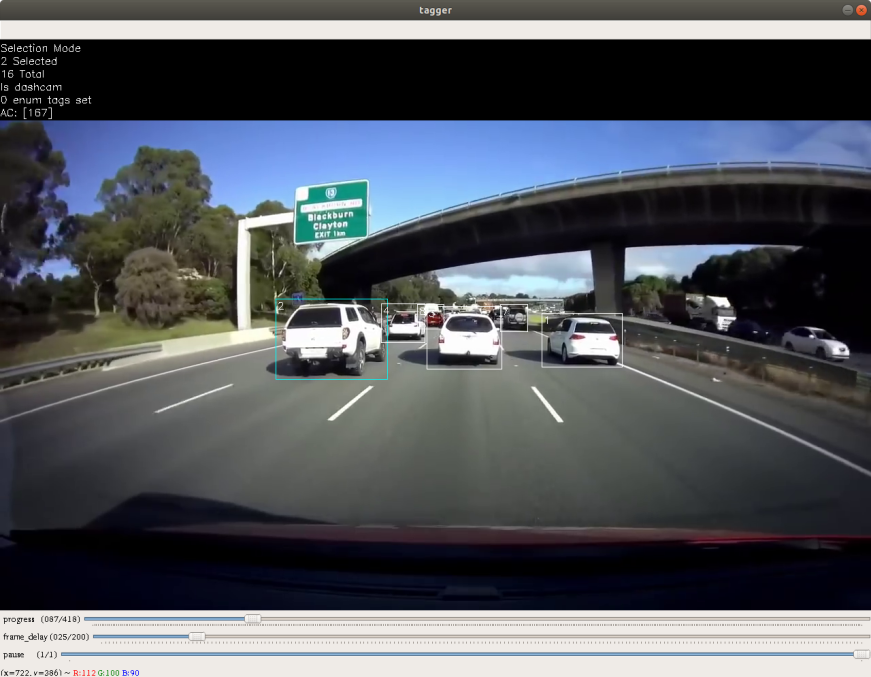
\includegraphics[width=0.5\textwidth]{example_gui_tool.png}
		\caption{GUI tool to facilitate annotation}
		\label{fig:example_gui_tool-png}
\end{figure}

%%%%%%%%%%%%%%%%%%%%%%%%%%%%%%%%%%%%%%%%%%%%%%%%%%%%%%%%%%%%%%%%%%%%%%%%%%%%%%%%
\section{EXPERIMENT}

In order to evaluate the importance of acquiring data from multiple geographical locations and under varying driving conditions around the world, we have manually collected a dataset of 223 video clips on which we will test the existing collision anticipation model, DSARNN. This dataset is comprised of 97 positive and 126 negative videos. Most of these videos represent road scenes from North America, Europe and Russia which have noticeably different characteristics than those in Taiwan. To prepare our data we follow the steps outlined by Chan et. al \cite{chan2016anticipating}. Namely, we trim videos such that they are 5 seconds long, sampled at 20 FPS, and the collision occurs at frame 90. This trimming and sampling functionality is provided within the pipeline configuration \texttt{smallcorgi\_exporter.yml}. In our experiments we train the DSARNN model on features produced by running a pre-trained VGG on each full frame and the cropped objects within the frame \cite{DBLP:journals/corr/SimonyanZ14a}. This is denoted VGG+RNN+F+D-con. in the original publication. We note that this data includes manually annotated bounding boxes, so there will be no error imposed by using automated vehicle detection and localization models.

In our first experiment we merge our dataset with the dataset provided by Chan et. al. We augment their training set with 77 positives and 106 negatives, and their testing set with 20 positives and 20 negatives. We use the same training procedure as Chan et. al, namely we train for 40 epochs with a learning rate of $10^{-4}$ and a batch size of 10. Although our data contribution here is relatively small, we observe a mean time-to-collision of 2.198s at 80\% recall which is very similar to the existing results from Chan et. al. However, we observe an average precision of 66.22\% which is appreciably lower than the 73.53\% average precision reported by Chan et. al. \cite{chan2016anticipating}

In our second experiment we use the provided pre-trained DSARNN model and test the performance on our entire dataset of 223 videos. We see very poor prediction performance at an average precision of 34.29\%, and in Figure \ref{fig:pr_curve} we observe poor precision at all recall values.

\begin{figure}[htpb]
		\centering
		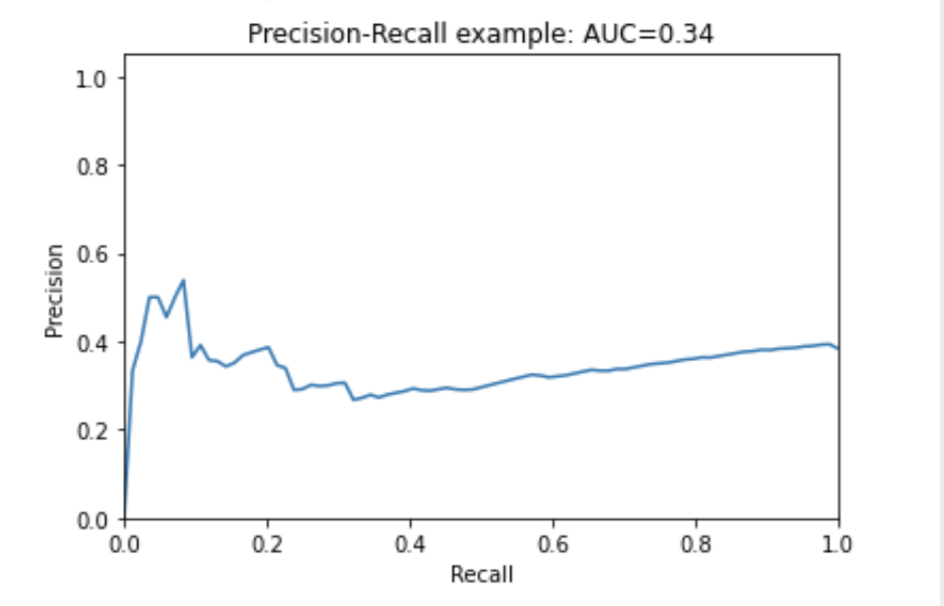
\includegraphics[width=0.4\textwidth]{prcurve.png}
		\caption{\todo{Write caption, fix label (I don't think the term AUC is correct here since this value is actually the average precision from the training code)}}
		\label{fig:pr_curve}
\end{figure}

These experiments seem to support the notion that in order for a collision prediction model to be generally effective in practice, it must be trained on collisions and complex roads scenes from varying regions and road conditions around the world, which is what we hope to achieve with this data collection pipeline.






\pgfplotstableread[col sep=comma]{by-classes.csv}\byclass
\pgfplotstableread[col sep=comma]{by-actors.csv}\byactors
\pgfplotstableread[col sep=comma]{by-agents.csv}\byagents
\pgfplotstableread[col sep=comma]{by-duration.csv}\byduration

We have aggregated some statistics about our dataset to help clients understand various distributions in the data. While these distributions may be representative of online collision footage, they are not necessarily representative of real world collisions. 

\begin{figure}[htpb]
		\centering
    \begin{tikzpicture}
    \begin{axis}[
      title={Objects by class},
      ylabel={Frequency (\# of objects)},
      xtick=data,
      xticklabels from table={\byclass}{X},
      xticklabel style={rotate=90}
    ]
    \addplot[fill, ybar] table [x expr=\coordindex, y={Y}] \byclass;
    \end{axis}
    \end{tikzpicture}
		\caption{Object by classes in our database}
		\label{fig:obj-by-class}
\end{figure}

\begin{figure}[htpb]
		\centering
    \begin{tikzpicture}
    \begin{axis}[
      title={Videos by participant},
      xlabel={Number of participants},
      ylabel={Frequency (\# of videos)},
      xtick=data,
      xticklabels from table={\byactors}{X}
    ]
    \addplot[fill, ybar] table [x expr=\coordindex, y={Y}] \byactors;
    \end{axis}
    \end{tikzpicture}
		\caption{Videos by number of participants}
		\label{fig:vids-by-participant}
\end{figure}

\begin{figure}[htpb]
		\centering
    \begin{tikzpicture}
    \begin{axis}[
      title={Videos by agents},
      xlabel={Number of agents},
      ylabel={Frequency (\# of videos)},
      xtick=data,
      xticklabels from table={\byagents}{X}
    ]
    \addplot[fill, ybar] table [x expr=\coordindex, y={Y}] \byagents;
    \end{axis}
    \end{tikzpicture}
		\caption{Videos by number of agents}
		\label{fig:vids-by-agents}
\end{figure}

\begin{figure}[htpb]
		\centering
    \begin{tikzpicture}
    \begin{axis}[
      title={Videos by duration},
      xlabel={Duration (in frames)},
      ylabel={Frequency (\# of videos)},
      xtick=data,
      xticklabels from table={\byduration}{X}
    ]
    \addplot[fill, ybar] table [x expr=\coordindex, y={Y}] \byduration;
    \end{axis}
    \end{tikzpicture}
		\caption{Videos by duration}
		\label{fig:vids-by-duration}
\end{figure}

\begin{figure}[htpb]
		\centering
    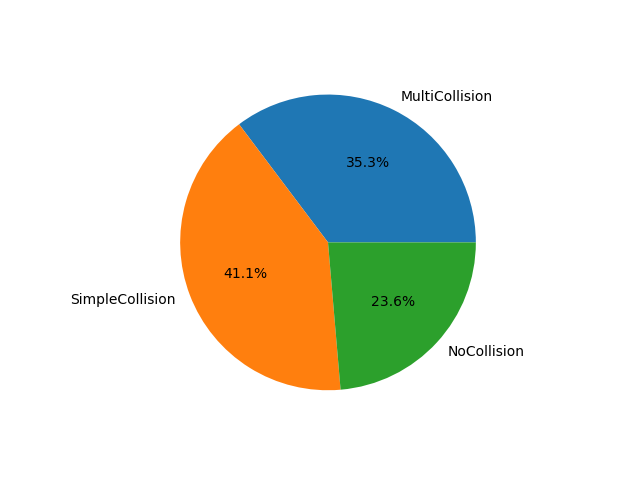
\includegraphics[width=3in]{by-collision.png}
		\caption{Videos by collision}
		\label{fig:vids-by-collision}
\end{figure}

\begin{figure}[htpb]
		\centering
    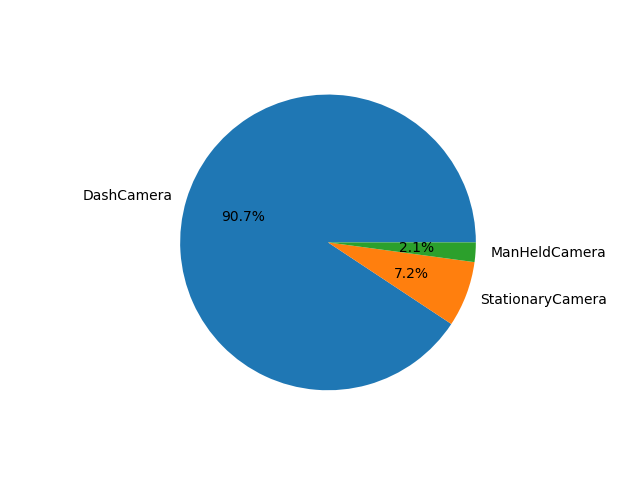
\includegraphics[width=3in]{by-camera.png}
		\caption{Videos by camera}
		\label{fig:vids-by-camera}
\end{figure}


%%%%%%%%%%%%%%%%%%%%%%%%%%%%%%%%%%%%%%%%%%%%%%%%%%%%%%%%%%%%%%%%%%%%%%%%%%%%%%%%
%\section{CONCLUSION}
% REMOVED BECAUSE WE DON'T HAVE ANY RESULTS
%\todo{Write the conclusion}
%A conclusion section is not required. Although a conclusion may review the main points of the paper, do not replicate the abstract as the conclusion. A conclusion might elaborate on the importance of the work or suggest applications and extensions.

%%%%%%%%%%%%%%%%%%%%%%%%%%%%%%%%%%%%%%%%%%%%%%%%%%%%%%%%%%%%%%%%%%%%%%%%%%%%%%%%
\section{FUTURE WORK}

There are many ways that we could improve our system, such as the following:
\begin{enumerate}
\item Custom interpolation between input frames: One idea would be to make it easier to modify the method of interpolation between frames. Currently, linear interpolation is always used. Moreover, given a type of interpolation is stored in the metadata, we probably shouldn't store all interpolated frames, rather than just the ones the user has entered. While linear interpolation works great for entering a frame every 10 frames, supporting more interpolations could be great for faster data entry, or even for supporting affine transformations on more complex bounds.

\item Polyhedral bounds: It's always possible to represent a 2-dimensional polyhedron with a matrix $A\in\mathbb{R}^{n\times 2}$, and a vector $b\in\mathbb{R}^2$, given that the polyhedron can be represented by the set $\left\{x\mid Ax\leq b\right\}$. We could use this idea to store masking bounds that can be used for training Mask-RCNN networks in (near-)collision contexts. 

\item Automated labelling: It would make labelling much faster if we had a (semi-)automated process of detecting objects and tracking them over frames. There are models for object detection that behave reasonably well which we could use, but they would still need to be augmented by a review process. For object tracking, there are simple heuristic algorithms that could be used. 

\item Web interface: Having a web-based user interface would be advantageous for this project. While currently being used in the context of (near-)collision, this software has the potential to become a platform for scraping automation and collaboration. Ideally, people without a technical background would be able to contribute to the microtasking involved, and technical contributors would be in charge of creating and managing the automation and general design of the pipeline.

\end{enumerate}

\addtolength{\textheight}{-12cm}

%%%%%%%%%%%%%%%%%%%%%%%%%%%%%%%%%%%%%%%%%%%%%%%%%%%%%%%%%%%%%%%%%%%%%%%%%%%%%%%%


\nocite{*}
\printbibliography

\end{document}
